\section{Live Testing}
\label{chap:live-test}

Despite the poor results from \autoref{chap:backtesting}, a strategy will be executed live on a demo account at ByBit for further development.
The primary purpose of this live test is not to achieve profitability but rather to validate the end-to-end functionality of the trading infrastructure under realistic market conditions.


\subsection{Broker Setup}

To connect to ByBit, the \texttt{ByBit Broker Connector} and \texttt{ByBit Remote DataSource} components have been used.

The \texttt{ByBit Remote DataSource} is able to:

\begin{enumerate}
    \item Request historical market data via the ByBit \texttt{Get Kline} API endpoint \cite{get-kline}.
    \item Stream market data through the ByBit \texttt{Kline} websocket endpoint \cite{stream-kline}.
\end{enumerate}

\noindent
The \texttt{ByBit Broker Connector} is able to execute the following actions via the ByBit API:

\begin{enumerate}
    \item Request the current wallet balance as well as the current margin \cite{wallet-balance}.
    \item Place orders in the market, which include open, take-profit, and stop-loss orders.
    Each Order is supported as limit and market order \cite{place-order}.
    \item Request all open positions for one or multiple pairs \cite{position-info}.
    In this paper, this only includes positions on \ethusdc.
    \item Request closed trades within a specified time period \cite{closed-pnl}.
\end{enumerate}

\noindent
The connection to ByBit is established by an API key and an API secret, which can be created in the ByBit web interface.
The distinction between a demo account and a real money account is regulated by ByBit via the base URL, which differs in each case.
To use the demo account, for REST endpoints, the base url \texttt{https://api-testnet.bybit.com} must be used.
For the real money account, the base url \texttt{https://api.bybit.com} must be used \cite{integration}.
To stream the market data, no distinction is required because the base URL \texttt{wss://stream.bybit.com/v5/public/linear} \cite{ws-connect} for streaming market data is a public endpoint that can be used without an API key.
In the trading engine, the base URLs, API key, and API secret are set via environment variables to achieve an independent implementation, configured by the user.

\subsection{Live-Test Results}

Using the trading engine configuration described above, a live execution of the triple exponential moving average strategy was performed from \liveStartDataStartDate~to \liveStartDataEndDate.
To keep the environment as similar as possible to the local backtest environment, the balance of the demo account was set to 5000 USDC at startup.

\begin{table}[H]
    \centering
    \centering
\begin{tabular}{ll|c}
    \toprule
    \multicolumn{2}{l|}{Strategy} & Triple EMA \\
    \midrule
    \multicolumn{2}{l|}{\textbf{Number of Trades}} & 66 \\
    \multicolumn{2}{l|}{\textbf{Maximum Gain}} & 304 \\
    \multicolumn{2}{l|}{\textbf{Maximum Loss}} & -228 \\
    \multicolumn{2}{l|}{\textbf{Profits Std.}} & 82 \\
    \multirow{3}{*}{\textbf{Equity}} & \textbf{Minimum} & 3640 \\
    & \textbf{Maximum} & 5000 \\
    & \textbf{Last}    & 3913 \\
    \multicolumn{2}{l|}{\textbf{Maximum Drawdown}} & 27 \\
    \multicolumn{2}{l|}{\textbf{Win Ratio}} & 27 \\
    \bottomrule
\end{tabular}

    \caption{Live-Test Statistics}
    \label{tbl:live-results}
\end{table}

\begin{figure}[H]
    \centering
    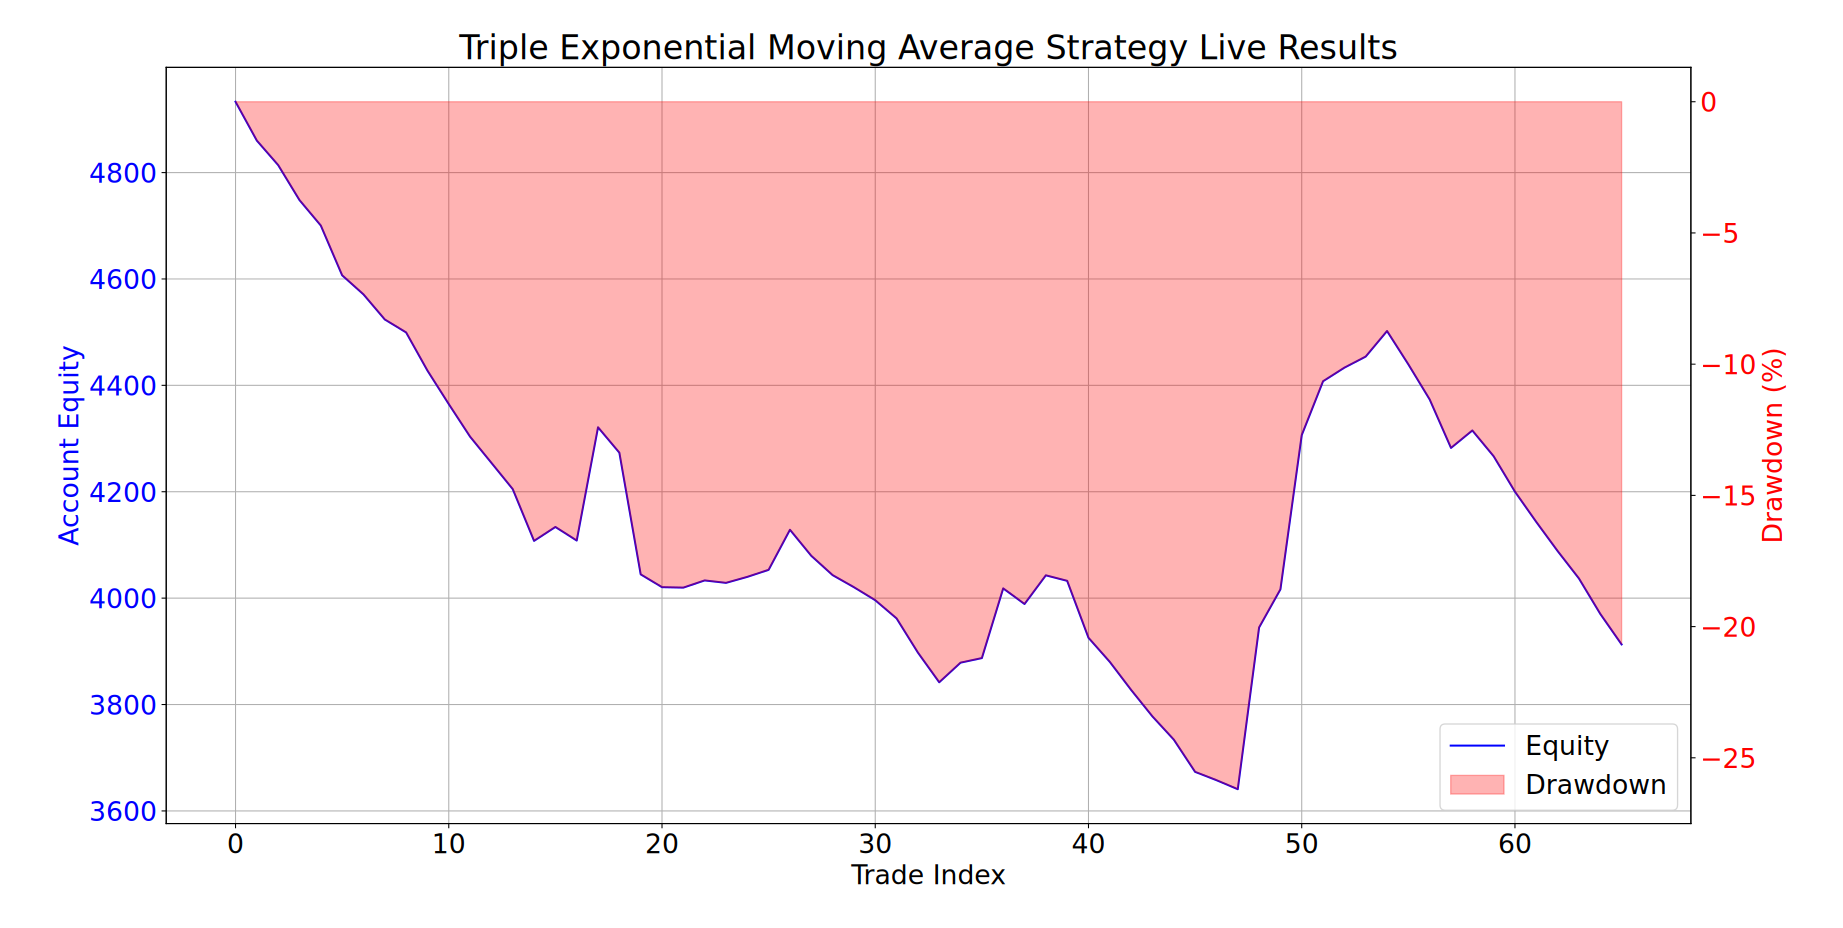
\includegraphics[width=\textwidth]{images/live/live-result}
    \caption{Live-Test Results}
    \label{fig:live-results}
\end{figure}

\noindent
As \autoref{tbl:live-results} and \autoref{fig:live-results} show, the strategy does not deliver profitable results in the live test either.

The logs \footnote{The logs are not published in this work due to their length.} show that the connection (data streaming) was interrupted several times during execution by the broker or due to network problems.
In these cases, the trading engine attempts to reconnect every ten seconds.
As soon as the connection is re-established, the engine continues to run normally.
The only limitation is that the internal state of the currently executing strategies is not reset, as this function does not yet exist.
This is particularly relevant if a connection interruption causes several candles to be skipped, making it appear to the strategies as if there were a jump in the data.
A mechanism must therefore be built in that detects gaps in the data and resets the strategies.
In the test carried out, however, this did not pose a problem, as the connection interruptions never lasted longer than a few seconds and no candles were missed.
